\section{netReplica}

\textbf{Changing section name and position in future}: 
\begin{itemize}
    \item netReplica architecture
    \item controlling the bandwidth  
    \item realistic background traffic 
    \item pinot nodes with different distance  
    \item controlling the bottleneck in access link
\end{itemize}



In order to create realistic network conditions, we need to be able to control the bandwidth and the background traffic plus running controlled applications. 
For traffic shaping, we use the LibreQoS open-source framework. LibreQoS is employed by many ISPs to control and monitor their networks, manage subscription plans, 
and provide optimal internet services to customers. It is scalable, having been tested with over 1000 users and 25+ Gbps, and is known for its low overhead. 
LibreQoS performs shaping and policing by relying on Linux's TC command and utilizing CAKE/FQ-CoDel active queue management. With LibreQoS, you can set minimum 
and maximum download/upload bandwidth for individual users or subnets in the network. We utilize this methodology to effectively shape and manage network traffic

\begin{figure}[H]
    \centering
    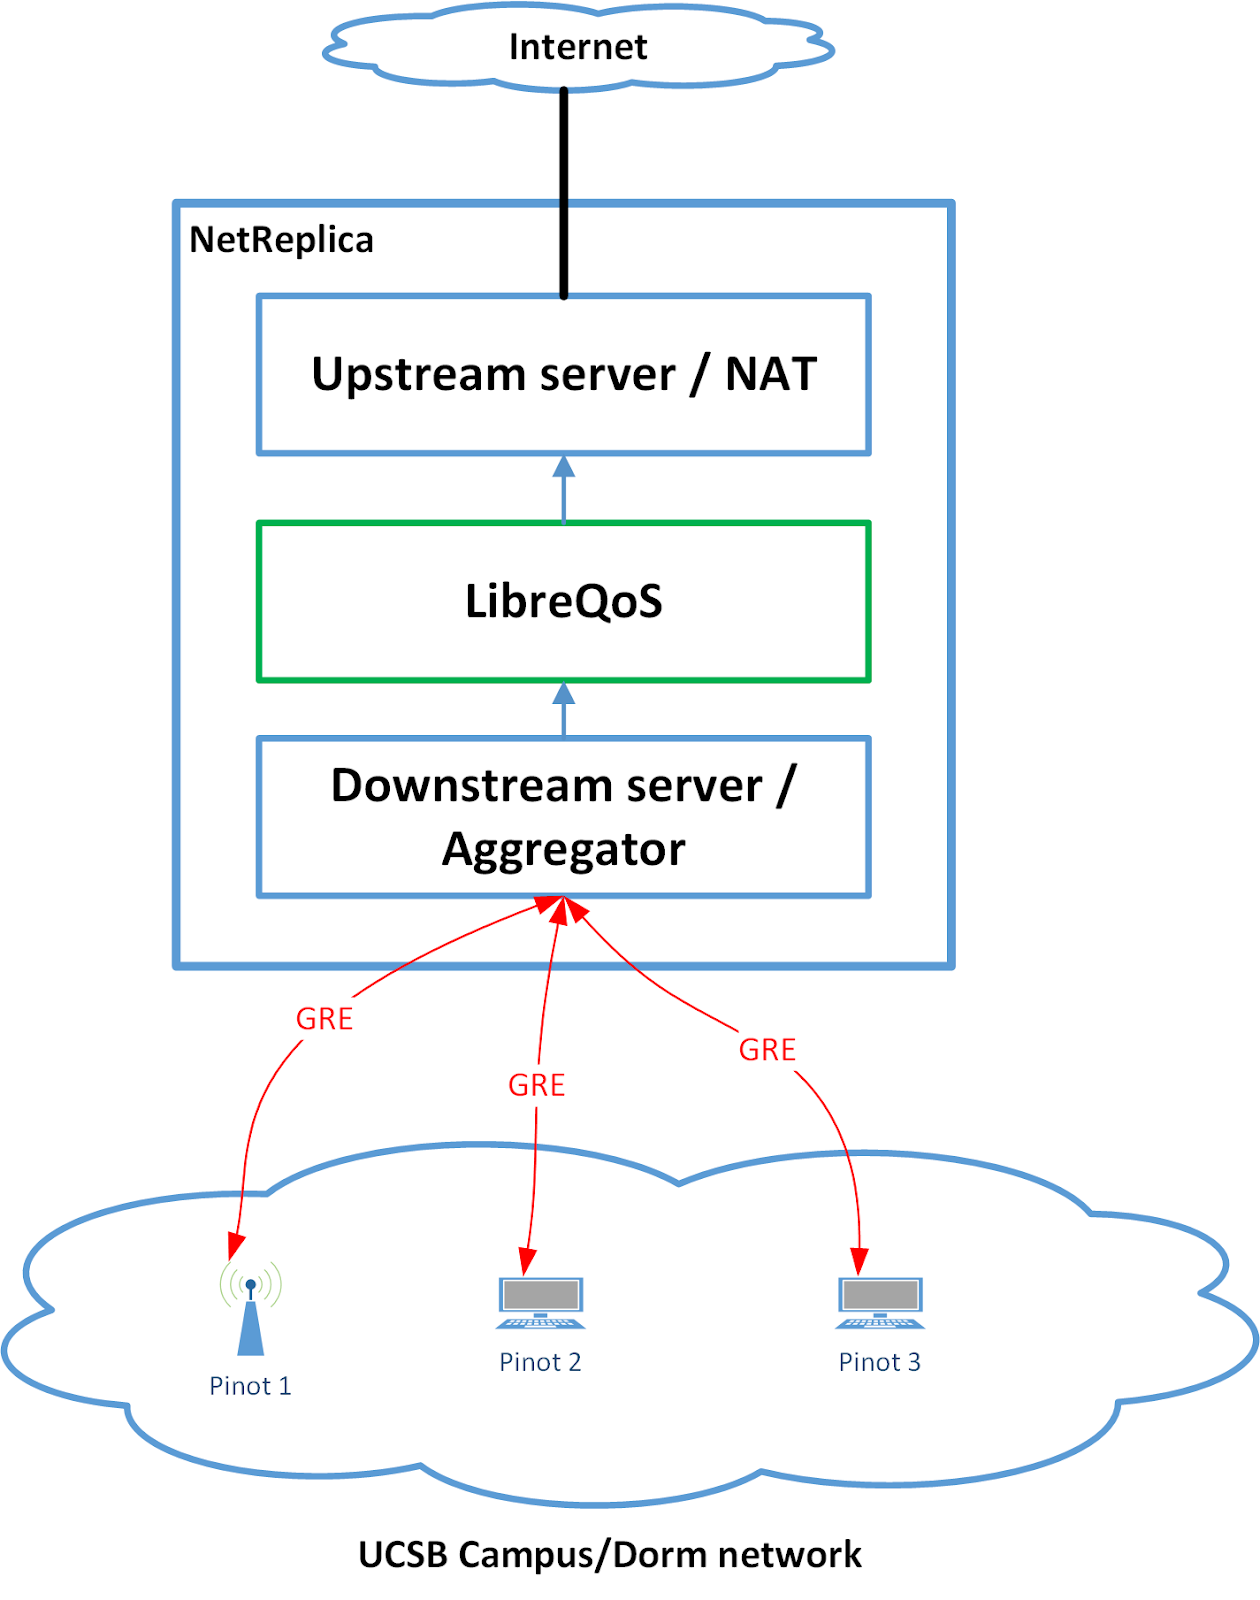
\includegraphics[width=0.8\textwidth]{figures/netReplica.png}
    \caption{netReplica Architecture}
    \label{fig:netReplica}
\end{figure}



Controlling available bandwidth alone does not accurately replicate real network conditions. Each hop from source to destination encounters background traffic from other users sharing network resources. For instance, in a home network, family members using the internet simultaneously can limit bandwidth and increase latency. The same applies to enterprise networks and ISPs, where multiple users access services concurrently, affecting application behavior and packet traces.
Realistic background traffic is crucial for accurate network condition simulation. In applications like video streaming, Adaptive Bitrate (ABR) algorithms may choose lower bitrates to prevent rebuffering under heavy network load. Even if application logic remains unchanged, packet traces are still affected; some packets experience more delay, interarrival times and the number of retransmissions may vary, and other metrics can also be impacted.
For these reasons, a realistic platform controlling network conditions must incorporate authentic background traffic that mimics real-world scenarios.

\subsection{Existing Approaches}
\begin{enumerate}
    \item No Background Traffic: Some studies neglect background traffic, resulting in datasets that fail to capture realistic traces and experiments.
    \item Steady Stream of Flows: Some studies use tools like iperf to create a steady stream of  background traffic with specific throughput. This method fails to represent the bursty nature of real network traffic.
    \item Probabilistic Models: Using Gaussian, Laplacian, or other distributions to generate bursty background traffic is an improvement. However, these models do not reflect real user behavior, as the bursts are not based on actual network traffic distributions.
    \item Trace-based Methods: Some approaches derive traffic distribution from input traces captured from real users using the internet and attempt to mimic it. While better, these methods often rely on simulation environments like MahiMahi, which have their own limitations. These limitations are discussed in subsequent sections.
\end{enumerate}

To create realistic background traffic that accurately mimics real user behavior, we use UCSB network traffic as background traffic. We select a subset of the captured traffic and replay it using the tcpreplay tool in our system while running the controlled application. 
We first captured traffic from the UCSB campus network, including dormitories, at the gateway of UCSB AS for 15 minutes. We collected MAC, IP, and transport layer headers, truncating payloads for privacy and performance while retaining the original packet length. Using PacketSplitter, we separated the captured data based on flows identified by 5-tuples and grouped them by internal IP address. Given that UCSB is one of the early hubs of the internet and has a large block of public IPv4 addresses, most users have unique public addresses, and there is limited network address translation (NAT) in place.
Next, we used CICFlowMeter to extract features from each flow pcap. Our tool, UserActivityAnalyzer (UAA), then analyzed user behavior based on CICFlowMeter output for all flows associated with each user. The extracted metrics included total forward/backward bytes, throughput, number of unique ports used, and distribution of active and idle times, among others.



\subsection{Experiment Design}
We are considering 3 different scenarios to evaluate the performance of this system using netReplica. 
\begin{itemize}
    \item Scenario 1: Wired vs. Wireless nodes 
    \item Scenario 2: Nodes with different distances to the bottleneck 
    \item Scenario 3: Limiting the bandwidth vs. not limiting the bandwidth
    \item Scenario 4: With/without background traffic
    \item scenario 5: Low burst background traffic vs. High burst background traffic
    \item scenario 6: Creating congestion in the access link 
    \item scenario 7: Utilizing different AQM algorithms at the bottleneck link
    \item scenario 8: Separating shaping bottleneck and background traffic bottleneck
\end{itemize}